% THIS IS SIGPROC-SP.TEX - VERSION 3.1
% WORKS WITH V3.2SP OF ACM_PROC_ARTICLE-SP.CLS
% APRIL 2009
%
% It is an example file showing how to use the 'acm_proc_article-sp.cls' V3.2SP
% LaTeX2e document class file for Conference Proceedings submissions.
% ----------------------------------------------------------------------------------------------------------------
% This .tex file (and associated .cls V3.2SP) *DOES NOT* produce:
%       1) The Permission Statement
%       2) The Conference (location) Info information
%       3) The Copyright Line with ACM data
%       4) Page numbering
% ---------------------------------------------------------------------------------------------------------------
% It is an example which *does* use the .bib file (from which the .bbl file
% is produced).
% REMEMBER HOWEVER: After having produced the .bbl file,
% and prior to final submission,
% you need to 'insert'  your .bbl file into your source .tex file so as to provide
% ONE 'self-contained' source file.
%
% Questions regarding SIGS should be sent to
% Adrienne Griscti ---> griscti@acm.org
%
% Questions/suggestions regarding the guidelines, .tex and .cls files, etc. to
% Gerald Murray ---> murray@hq.acm.org
%
% For tracking purposes - this is V3.1SP - APRIL 2009

\documentclass{acm_proc_article-sp}

\usepackage{url}

\begin{document}

\title{Title}
%\subtitle{[Extended Abstract]
%\titlenote{A full version of this paper is available as
%\textit{Author's Guide to Preparing ACM SIG Proceedings Using
%\LaTeX$2_\epsilon$\ and BibTeX} at
%\texttt{www.acm.org/eaddress.htm}}}
%
% You need the command \numberofauthors to handle the 'placement
% and alignment' of the authors beneath the title.
%
% For aesthetic reasons, we recommend 'three authors at a time'
% i.e. three 'name/affiliation blocks' be placed beneath the title.
%
% NOTE: You are NOT restricted in how many 'rows' of
% "name/affiliations" may appear. We just ask that you restrict
% the number of 'columns' to three.
%
% Because of the available 'opening page real-estate'
% we ask you to refrain from putting more than six authors
% (two rows with three columns) beneath the article title.
% More than six makes the first-page appear very cluttered indeed.
%
% Use the \alignauthor commands to handle the names
% and affiliations for an 'aesthetic maximum' of six authors.
% Add names, affiliations, addresses for
% the seventh etc. author(s) as the argument for the
% \additionalauthors command.
% These 'additional authors' will be output/set for you
% without further effort on your part as the last section in
% the body of your article BEFORE References or any Appendices.

\numberofauthors{3} %  in this sample file, there are a *total*
% of EIGHT authors. SIX appear on the 'first-page' (for formatting
% reasons) and the remaining two appear in the \additionalauthors section.
%
\author{
% You can go ahead and credit any number of authors here,
% e.g. one 'row of three' or two rows (consisting of one row of three
% and a second row of one, two or three).
%
% The command \alignauthor (no curly braces needed) should
% precede each author name, affiliation/snail-mail address and
% e-mail address. Additionally, tag each line of
% affiliation/address with \affaddr, and tag the
% e-mail address with \email.
%
% 1st. author
\alignauthor
Maximilian Klein\\%\titlenote{Dr.~Trovato insisted his name be first.}\\
       %\affaddr{School of Information}\\
       %\affaddr{ University of California, Berkeley, 102 South Hall}\\
       %\affaddr{Berkeley, CA 94720}\\
       \email{confusing@notconfusing.com}
% 2st. author
\alignauthor
Thomas Maillart\\%\titlenote{Dr.~Trovato insisted his name be first.}\\
       \affaddr{School of Information}\\
       \affaddr{ University of California, Berkeley, 102 South Hall}\\
       \affaddr{Berkeley, CA 94720}\\
       \email{thomas.maillart@ischool.berkeley.edu}
% 3rd. author
\alignauthor
John Chuang\\%\titlenote{Dr.~Trovato insisted his name be first.}\\
       \affaddr{School of Information}\\
       \affaddr{ University of California, Berkeley, 102 South Hall}\\
       \affaddr{Berkeley, CA 94720}\\
       \email{chuang@ischool.berkeley.edu}
}





\date{30 July 1999}
% Just remember to make sure that the TOTAL number of authors
% is the number that will appear on the first page PLUS the
% number that will appear in the \additionalauthors section.

\maketitle
\begin{abstract}
Abstract
\end{abstract}

% A category with the (minimum) three required fields
\category{H.4}{Information Systems Applications}{Miscellaneous}
%A category including the fourth, optional field follows...
\category{D.2.8}{Software Engineering}{Metrics}[complexity measures, performance measures]

\terms{to be completed}

\keywords{to be completed, if necessary} % NOT required for Proceedings

\section{Introduction}

3 elements. Literature. Question. Data. The need for a new metric.

2. We also inadvertently develop a new measure for the convtroversialness of articles, and the collaborativeness of a group of editors.

4. We need an intuitive way of understanding the iterative algorithm

We then applied the most general implementation of the $\mathbf{FQ}$ algorithm as developed for modelling the economy and competitiveness of countries. The $\mathbf{FQ}$ is a nonlinear generalization of the Hidalgo Hausman "Reflections Method". \cite{Caldarelli}. The algorithm has both a stochastic, iterative implementation, and an analytic solution. We demonstrate the iterative solution, to gain some intuition for the algorithm.

$ w^*_c = A(\sum^{N_p}_{p=1} M_{cp}k_p^{-\alpha})k_c^{-\beta}$

$ w^*_p = B(\sum^{N_c}_{c=1} M_{cp}k_c^{-\beta})k_p^{-\alpha}$

At each iterative step we simultaneously rank editor "fitness", and article "ubiquity". In the linear model, the first iteration of "fitness" is the sum of articles to which that editor has contributed, and the "ubiquity" is the sum of editor who have contributed to that article. In the second iteration, say a user is as fit as the average the ubiquities of the of the pages edited. But this is all things being equal.

In the economic domain, the best products are those that are made by the fewest countries. Therefore in our average we want to give more weight to those best producing countries. This measure of good contributors being more important to success, is measured by alpha. A higher alpha means that a good product needs to be exported by the best countries. In Caldarelli, to correlate best with GDP rankings alpha = 1.5 Our result we find the  opposite - negative values of alpha. in the not competitive but collaborative wikipedia, where the best articles are produced by the highest number of editors

 

\section{Method}

1. The current investigation involved collecting historical data of edition and quality metrics, from 10 categories of articles in English Wikipedia, with focus on fine-grained edits by contributors to articles.

2. The chosen categories contain between 50 and 4000 articles, and between 50 and 5000 contributors have edited at least 100'000 times all the articles over their history. (c.f. table \ref{tab:statistics} for summary statistics on the categories). 

3. For each category, we constructed 10 accumulative snapshots, that is each starting from the first edit in the category until 10\% more of the categories total edits have occurred. \ref{fig:accumulative_snapshots}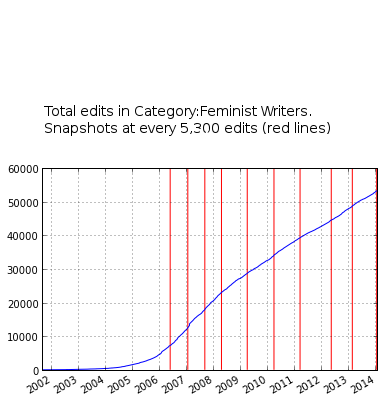
\includegraphics[scale=1]{accumulative snapshot points for Feminist Writers.png}. For each snapshot, we constructed the matrix $\mathbf{M_{e,a}}$ of contributors versus edited articles, similar to the country versus products matrix of the Economics Domain. For each snapshot, the values in $\mathbf{M_{e,a}}$ are defined as the number of edits made by editor $e$ on article $a$ in the category occurring in the snapshot time. Note that the final snapshot represents the entire history of the category up to the present date. 

The matrix $\mathbf{\hat{M}_{e,a}}$ is a binary representation of $\mathbf{M_{e,a}}$ where each nonzero entry is replaced with $1$. This represents if editors have touched which articles rather than how much they have touched each article. In the economics domain, the distinction of making a binary matrix out of the data is interpreted an alternative metric to GDP per capita, rather than GDP. Here we could also see the distinction as normalized editor fitness.

It has a typical triangular structure as shown on Figure \ref{fig:triangular_matrix}.

The matrix $\mathbf{\hat{M}_{e,a}}$ constitutes the basic input for implementing the Biased Markov Chain Approach, which we will call the $\mathbf{w^*}$ algorithm, which is an analytic solution to the iterative $\mathbf{W}$ algorithm. \cite{Caldarelli} 

In the iterative solution we see how certain editors start low, but then climb in rankings. This means that they are editing few articles, but those articles are of higher quality. Likewise certain articles climb over iterations, they are edited by relatively few editors, but those editors are fitter.

The output of $\mathbf{w^*}$ are a pair of rankings $ w^*_e$ and $ w^*_a$ for editors and articles respectively.

$w^*_e = A(\sum^{N_a}_{a=1} M_{e,a}k_a^{-\alpha})k_e^{-\beta}$

$w^*_a = B(\sum^{N_e}_{e=1} M_{e,a}k_e^{-\beta})k_a^{-\alpha}$]

Next we collect exogenous metrics as comparison for both  $w^{*}_{e}$ and $w^{*}_{a}$, which we call  $v_e$ and $v_a$.

The exogenous metric for editors $v_e$ we take is $labour hours$. For each editor the contribution history upto the snapshot point,  divide into strings of $edit sessions$, edits that occur within 1 hour of the previous edit. Then $labour hours$ are determined by subtracting the looking at the total time between the first and last edit in each edit session, and then summing the labours of each edit session. \cite{Geiger, Halfaker}. 

For an exogenous measure of article quality, $ v_a$,  we use a group of 5 text analysis metrics performed on Wikipedia articles at the lastest time in the snapshot. These are ratio of mark-up to readable text, number of headings, article length, citations per article length, and outgoing intrawiki links. To reduce the dimensionality of these 5 metrics, we perform Principal Component Analysis, and accept the principal component. Variance explained by the first principal component, was as high as .7 and never below .5 http://www-users.cs.umn.edu/~morten/publications/wikisym2013-tellmemore.pdf, http://mailer.fsu.edu/~bstvilia/papers/quantWiki.pdf \cite{ Morten}.


\subsection{Calibrating}

Having our endogenous and exegenous variables now, we perform a recursive grid search over the two dimensions of \alpha and \beta to find a maximum correlation between our rankings from $\mathbf{w^*}$ and our exogenous variables. Our grid search operates on the interval $[-5,5]$ with a resolution of 0.2 in on each axis. Importantly we search for negative values of \alpha and \beta, which is not done in the Economics Domain. t

\subsection{Finding trends}

5. While the implementation presented here is strictly similar to \ref{}, the interpretation is slightly different in the context of group collaboration. Indeed, while countries competes for selling products, the hypothesis here is that Wikipedia contributors cooperate, at least in a very informal way, for improving the quality of articles.

\section{Results}

\section{Discussion}

6. {\it Refer to problems here, if any.}

\begin{table}
\centering
\caption{Summary statistics for each category}
\begin{tabular}{|c|c|l|} \hline
Non-English or Math&Frequency&Comments\\ \hline
\O & 1 in 1,000& For Swedish names\\ \hline
$\pi$ & 1 in 5& Common in math\\ \hline
\$ & 4 in 5 & Used in business\\ \hline
$\Psi^2_1$ & 1 in 40,000& Unexplained usage\\
\hline\end{tabular}
\label{tab:statistics}
\end{table}


\begin{figure}
\centering
%\epsfig{file=fly.eps}
\caption{Matrix $\mathbf{M}$ ordered by decreasing order of edits on both contributors and articles dimensions.}
\label{fig:matrix}
\end{figure}

\section{Conclusions}

%ACKNOWLEDGMENTS are optional
%\section{Acknowledgments}

%
% The following two commands are all you need in the
% initial runs of your .tex file to
% produce the bibliography for the citations in your paper.
\bibliographystyle{abbrv}
\bibliography{sigproc}  % sigproc.bib is the name of the Bibliography in this case
% You must have a proper ".bib" file
%  and remember to run:
% latex bibtex latex latex
% to resolve all references
%
% ACM needs 'a single self-contained file'!
%
%APPENDICES are optional
%\balancecolumns
%\appendix
%Appendix A
%\section{Headings in Appendices}

\end{document}
